\section{Mallado (Mesh)}

En esta sección veremos cómo se generan las mallas en OpenFOAM y mencionaremos algunas herramientas externas, como la importación de geometrías desde FreeCAD.

\subsection{Generación}

En OpenFOAM la estructura de malla se conoce como \texttt{polyMesh}. Para empezar a construir cualquier geometría necesitamos entender de qué está compuesta.
\begin{itemize}
  \item \textbf{Puntos}: están colocados en el espacio 3D, definidos por un vector $(x, y, z)$, y se enumeran en el orden en que aparecen comenzando desde cero. En la lista no puede haber puntos con las mismas coordenadas ni algún punto que no esté contenido en alguna cara. Los denotaremos por $p_n$, donde $n$ es un número natural incluyendo el cero.
  \item \textbf{Caras}: es una lista ordenada de puntos, donde los puntos se referencian mediante su posición en el archivo. Para ir colocando los puntos de una cara tenemos que usar la regla de la mano derecha y, en ese orden, asignarlos. Existen dos tipos de caras:
    \begin{itemize}
      \item \textbf{Caras internas}: están conectadas a dos celdas.
      \item \textbf{Caras de frontera}: pertenecen a una sola celda y su vector normal debe apuntar hacia fuera del dominio computacional.
    \end{itemize}
  \item \textbf{Celdas}: es una lista de caras en orden arbitrario. Deben ser continuas (no deben encimarse), convexas (su centro debe estar dentro de la celda), cerradas y ortogonales.
  \item \textbf{Frontera}: es el conjunto de caras que delimitan el dominio y que se agrupan en parches (\textit{patches}) con un nombre y un tipo determinados.
\end{itemize}

Ahora que sabemos de qué se compone el mallado, podemos empezar a crear formas. Para esto tenemos que saber que las formas están definidas por el orden en que colocamos los puntos; este orden debe hacer que las figuras no sean degeneradas o estén retorcidas. Para esto primero ocupamos una lista de puntos de esta manera:
\begin{figure}[h]
  \centering
  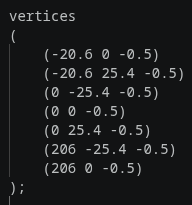
\includegraphics[width=0.3\linewidth]{puntos.png}
  \caption{Vértices del mallado}
\end{figure}

Una vez dada la lista de puntos para cualquier figura, tenemos que dar una lista de los puntos de esa figura. Debemos colocar estos puntos de manera que, si existe una arista entre dos puntos, estos aparezcan consecutivos en la lista.

Después tenemos que poner entre paréntesis cómo queremos que estas figuras sean divididas: $a$, $b$ y $c$ indican la división del bloque en cada dirección.
\begin{verbatim}
  (a b c)
\end{verbatim}

Veamos las formas que existen y cómo usarlas:

\begin{itemize}
  \item \textbf{Hexaedros}: para definir un hexaedro lo hacemos con:
    \begin{verbatim}
      hex (p1 p2 p3 ... p8) (a b c)
    \end{verbatim}

  \item \textbf{Wedge}: \texttt{wedge (p1 p2 p3 ... p7) (a b c)}

  \item \textbf{Prisma}: \texttt{prism (p1 p2 p3 ... p6) (a b c)}

  \item \textbf{Pirámide}: \texttt{pyr (p1 p2 p3 ... p5) (a b c)}

  \item \textbf{Tetraedro}: \texttt{tet (p1 p2 p3 ... p4) (a b c)}

  \item \textbf{Arista de tetraedro}: \texttt{tetWedge (p1 p2 p3 ... p5) (a b c)}
\end{itemize}

Para colocar cualquiera de estos debemos ponerlos dentro de algo llamado \texttt{blocks} de esta manera:
\begin{verbatim}
  blocks
  (
    hex (0 1 2 3 4 5 6 7) (1 1 1)
  );
\end{verbatim}
En este bloque van todas las figuras.

\subsection{Tipos de caras}

Esto nos define el comportamiento que tendrán las caras de las formas. Estas están divididas en los siguientes tipos:
\begin{itemize}
  \item \texttt{patch}: no contiene ninguna propiedad geométrica o topológica del mallado, pero sirve para \textit{inlet} u \textit{outlet}; no aporta información sobre la pared.
  \item \texttt{wall}: pared sólida dentro del dominio.
  \item \texttt{symmetryPlane}: replica lo que ocurre en el plano de simetría.
  \item \texttt{empty}: sirve para resolver mejor los casos en 2 dimensiones agregando la condición de \texttt{empty}.
\end{itemize}

Para colocar las caras debemos hacer lo siguiente:
\begin{verbatim}
  boundary
  (
    caras
    {
      type wall;
      faces
      (
        (0 1 2 3)
        (1 3 4 5)
      );
    }
  );
\end{verbatim}
donde \texttt{caras} es cualquier nombre y en \texttt{type} puede ir cualquiera de los tipos de la lista anterior.

\subsection{Compilar}

Para poder ver lo que hemos hecho tenemos que tener lo siguiente: la escala, que usualmente va al inicio y se ve así: \texttt{convertToMeters x;} o \texttt{scale x;}, donde $x$ es un número y esta es la escala de distancias. Después colocamos \texttt{vertices}, \texttt{blocks} y, por último, \texttt{boundary}.

Una vez que tenemos esto, podemos correr lo siguiente para compilar y visualizar:
\begin{verbatim}
  blockMesh
  paraFoam &
\end{verbatim}
Aquí \texttt{blockMesh} compila y \texttt{paraFoam} abre el visualizador para ver la malla.

\subsection{cfMesh}

\texttt{cfMesh} es una librería de código abierto para generación automática de mallas, desarrollada por Creative Fields. A diferencia de \texttt{blockMesh}, que requiere que el usuario defina manualmente los bloques, \texttt{cfMesh} puede generar mallas a partir de una geometría de superficie (STL) de forma casi automática.

Sus utilidades principales son:
\begin{itemize}
  \item \texttt{cartesianMesh}: genera una malla predominantemente hexaédrica a partir de una superficie triangulada. Es la opción más robusta y rápida para geometrías complejas.
  \item \texttt{tetMesh}: genera una malla tetraédrica, útil cuando la geometría tiene detalles muy pequeños que una malla hexaédrica no podría capturar bien.
  \item \texttt{pMesh}: genera una malla poliedral, que combina celdas de distintos tipos y suele reducir el número total de celdas.
\end{itemize}

El flujo de trabajo típico con \texttt{cfMesh} es:
\begin{enumerate}
  \item Preparar un archivo STL con la superficie del dominio.
  \item Crear un archivo \texttt{system/meshDict} con los parámetros de refinamiento y capas límite.
  \item Ejecutar la utilidad correspondiente, por ejemplo: \texttt{cartesianMesh}.
  \item Verificar la malla con \texttt{checkMesh}.
\end{enumerate}

\texttt{cfMesh} no viene incluido en la distribución estándar de OpenFOAM; debe compilarse e instalarse por separado.

\subsection{snappyHexMesh}

\texttt{snappyHexMesh} es la herramienta nativa de OpenFOAM para generar mallas 3D complejas a partir de una malla de fondo hexaédrica creada con \texttt{blockMesh}. Su funcionamiento se basa en tres etapas consecutivas:

\begin{enumerate}
  \item \textbf{Castellated mesh}: se parte de la malla de fondo y se eliminan las celdas que quedan fuera de la geometría (definida por un archivo STL). Las celdas cercanas a la superficie se refinan según los niveles especificados en \texttt{snappyHexMeshDict}.
  \item \textbf{Snap}: las celdas que quedaron cortadas por la superficie se ajustan (\textit{snap}) para que sus caras coincidan con la geometría. Aquí es donde se preservan las aristas vivas extraídas previamente con \texttt{surfaceFeatureExtract}.
  \item \textbf{Add layers}: se añaden capas límite (\textit{boundary layers}) cerca de la superficie para capturar correctamente los gradientes de velocidad en la pared, algo esencial para modelos de turbulencia de bajo número de Reynolds.
\end{enumerate}

El flujo de trabajo típico es:
\begin{verbatim}
  blockMesh
  surfaceFeatureExtract
  snappyHexMesh -overwrite
  checkMesh
\end{verbatim}

El archivo \texttt{system/snappyHexMeshDict} controla todos los parámetros: la geometría de entrada (\texttt{geometry}), los refinamientos locales (\texttt{refinementSurfaces}, \texttt{refinementRegions}), los parámetros de \textit{snapping} y la configuración de capas. Es un archivo extenso y su correcta configuración es uno de los aspectos más delicados del preprocesamiento en OpenFOAM.
